\section{Test}

Der Test, der hier detailliert beschrieben wird, wurde w"ahrend der Fachstudie
im Nexus-Labor mit der Test-Hardware durchgef"uhrt.

\subsection{Hardware}

Zuerst wurde folgende Hardware f"ur den Test im Nexus-Labor eingerichtet:
\begin{itemize}
\item Zwei Rechner (x86) mit jeweils einer \textbf{Wistron CM9 Atheros AR5213A}
(siehe \ref{Wistron CM9 Atheros AR5213A}) WLAN-Karte
\item Ein Laptop (x86) mit einer \textbf{Intel Wireless WiFi Link 4965AGN}
(siehe \ref{Intel Wireless WiFi Link 4965AGN}) WLAN-Karte
\end{itemize}

\begin{figure}[H]
  \centering
  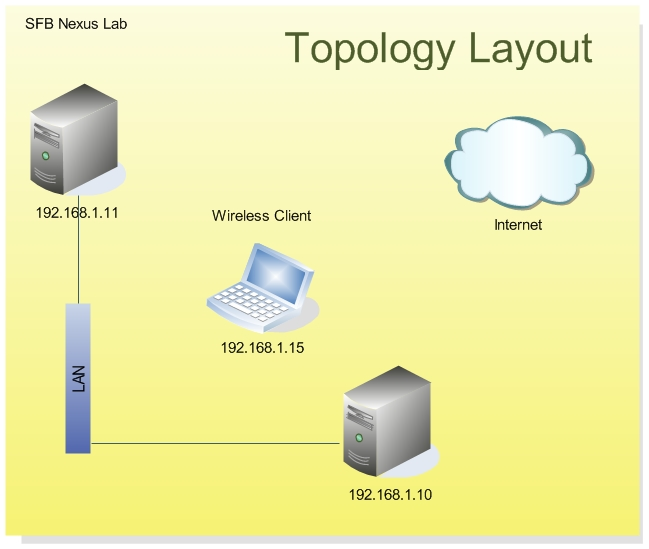
\includegraphics[width=0.8\textwidth]{images/Labor.jpg}
  \caption{Topologie}
  \label{fig:Topologie}
\end{figure}

\subsection{Software}

\subsubsection{Betriebssystem}

Auf den Rechnern mit der Wistron CM9 Atheros AR5213A WLAN-Karte wurde
als Betriebssystem Fedora 6 mit Linux Kernel 2.6.18
und auf dem Laptop Windows XP verwendet.

\subsubsection{Treiber f"ur WLAN-Karten}

In diesem Abschnitt wird beschrieben, wie man Treiber f"ur WLAN-Karten
auf den beiden Rechnern und Laptop installiert und die WLAN-Karten
konfiguriert werden k"onnen.

Auf den Rechnern mit der Wistron CM9 Atheros AR5213A WLAN-Karte
wurde die letzte Version des MadWifi-Treibers zuerst kompiliert und dann
installiert.

Kompilieren des MadWifi-Treibers:
\begin{shelllst}
svn checkout http://svn.madwifi.org/madwifi/trunk madwifi
cd madwifi
make
\end{shelllst}

Installieren des kompilierten MadWifi-Treibers (\textbf{root}-Rechte ben"otigt):
\begin{shelllst}
make install
\end{shelllst}

Manuelles Laden des MadWifi-Treibers (\textbf{root}-Rechte ben"otigt):
\begin{shelllst}
modprobe ath_pci
\end{shelllst}

Automastische Laden des MadWifi-Treibers beim Booten
(\textbf{root}-Rechte ben"otigt):
\begin{shelllst}
mkdir /etc/modules.autoload.d/
echo ath_pci >> /etc/modules.autoload.d/kernel-2.6
\end{shelllst}

Nachdem der MadWifi-Treiber geladen wurde (manuell oder automatisch),
kann die WLAN-Karte konfiguriert werden. Die WLAN-Karte kann entweder
manuell oder automatisch beim Booten konfiguriert werden.

Manuelles Konfigurieren der WLAN-Karte (\textbf{root}-Rechte ben"otigt):
\begin{shelllst}
ifconfig ath1 inet 192.168.2.1/24 # IP-Adresse
iwconfig ath1 essid mesh          # SSID="mesh"
iwconfig ath1 mode ad-hoc         # Ad-Hoc Modus einschalten
iwconfig ath1 channel 36          # 802.11a Kanal 36
iwconfig ath1 enc s:1234567890abc # 108 bit WEP-Passwort
                                  # (13 Zeichen)
\end{shelllst}

Damit die WLAN-Karte beim Booten von Fedora 6
automatisch konfiguriert werden kann, muss eine Konfigurationsdatei
mit dem Namen \textbf{ifcfg-ath1} im Verzeichnis
\textbf{/etc/sysconfig/network-scripts} angelegt werden.

Listing der Datei \textbf{/etc/sysconfig/network-scripts/ifcfg-ath1}:
\begin{shelllst}
cat /etc/sysconfig/network-scripts/ifcfg-ath1
DEVICE=ath1
ONBOOT=yes
			
BOOTPROTO=static
IPADDR=192.168.2.1
NETMASK=255.255.255.0
			
ESSID=mesh
MODE=ad-hoc
CHANNEL=36
KEY=s:1234567890abc
\end{shelllst}

Nachdem die Datei \textbf{/etc/sysconfig/network-scripts/ifcfg-ath1}
erstellt wurde, muss Init-Skripot f"ur Netzwerk-Dienste neugestartet
werden (\textbf{root}-Rechte ben"otigt):
\begin{shelllst}
/etc/init.d/network restart
\end{shelllst}

Den offiziellen Windows-Treiber f"ur die Intel Wireless WiFi Link 4965AGN
WLAN-Karte kann auf der Intel-Webpage heruntergeladen werden. Die Anleitung
zur Installation und Konfiguration diesr WLAN-Karte findet man auch
auf der selben Webpage (siehe \ref{Intel Wireless WiFi Link 4965AGN}) und
wird hier nicht weiter beschrieben.

\subsubsection{olsrd}

In diesem Abschnitt wird erkl"art, wie man den olsr.org OLSR daemon kompiliert,
installiert und konfiguriert. Au"serdem wird hier auch gezeigt, wie man
Plugins f"ur den olsr.org OLSR daemon kompiliert uns installiert.

Kompilieren des OLSR daemons:
\begin{shelllst}
cvs -d:pserver:anonymous@olsrd.cvs.sourceforge.net:\
	/cvsroot/olsrd login
cvs -z3 -d:pserver:anonymous@olsrd.cvs.sourceforge.net:\
	/cvsroot/olsrd co olsrd-current
cd olsrd-current
make
\end{shelllst}

Installieren des OLSR daemons (\textbf{root}-Rechte ben"otigt):
\begin{shelllst}
make install
\end{shelllst}

Im Folgenden wird demonstriert, wie man
das HTTP Mini-Server Plugin \textbf{httpinfo} kompiliert und installiert.
Das Plugin \textbf{httpinfo} ist ein kleiner und einfacher HTTP-Server und
erlaubt es, z.B. die Routing-Tabelle eines Knotens in einem Mesh-Netzwerk
zu erfassen.

Damit die Topology eines Mesh-Netzwerkes visualisiert werden kann,
muss noch das Dot Data Generation Plugin \textbf{dot\_draw}
kompiliert und installiert werden. Das Plugin \textbf{dot\_draw}
ist auch ein kleiner Server. Wenn man eine TCP-Verbindung zu diesem Server
aufbaut (z.B mit \textbf{netcat} oder \textbf{telnet}),
dann bekommt man die aktuelle Topology des Mesh-Netzwerkes in
Form eines Dot-Graphes
(siehe GrpahViz \url{http://www.graphviz.org} und
 \url{de.wikipedia.org/wiki/DOT\_(GraphViz)}).
Dieser Dot-Graph ist eine einfache Textdatei und kann mit Hilfe des
Programms \textbf{dot} zu einem Bild konvertiert werden.

Es gibt noch andere zahlreiche Plugins f"ur
den olsr.org OLSR daemon. Sie alle k"onnen auf dieselbe Weise kompiliert
und installiert werden.

Kompilieren des HTTP Mini-Server Plugins \textbf{httpinfo}:
\begin{shelllst}
cd lib/httpinfo
make
\end{shelllst}

Installieren des HTTP Mini-Server Plugins \textbf{httpinfo}
(\textbf{root}-Rechte ben"otigt):
\begin{shelllst}
make install 
chcon -t textrel_shlib_t /usr/lib/olsrd_httpinfo.so.0.1
\end{shelllst}

Der olsr.org OLSR daemon wird "uber die Datei \textbf{/etc/olsrd.conf}
konfiguriert.  Das vollst"andige Listing der Datei \textbf{/etc/olsrd.conf} ist
im Anhang angegeben (siehe \ref{olsrd.conf}).
Es muss vor allem das Netzwerk-Interface und Plugins konfiguriert werden.

Starten des olsr.org OLSR daemons
(\textbf{root}-Rechte ben"otigt):
\begin{shelllst}
olsrd
\end{shelllst}

Der olsr.org OLSR daemon kann auch automatisch beim Starten
des Betriebssystems gestartet werden. Daf"ur muss ein Startup-Skript
\textbf{/etc/init.d/olsrd} erzeugt werden. Das Listing der Datei
\textbf{/etc/init.d/olsrd} kann man hier betrachten \ref{olsrd_startup.sh}.

Nachdem die Date erzeugt wurde, muss noch das System so konfiguriert
werden, das das Startup-Skript \textbf{/etc/init.d/olsrd} beim Booten
ausgef"uhrt werden kann (\textbf{root}-Rechte ben"otigt):
\begin{shelllst}
chmod 755 /etc/init.d/olsrd
chkconfig --add olsrd
\end{shelllst}

Das Kompilieren und Konfigurieren des olsr.org OLSR daemons f"ur Windows XP
wird hier nicht erkl"art, weil es ziehmlich kompliziert ist. Wir haben
den olsr.org OLSR daemon und die GUI zu ihm f"ur Windows XP selbst kompiliert
und konfiguriert. Um den olsr.org OLSR daemon zu kompilieren, wird cygwin
mit gcc ben"otigt. Um die GUI f"ur den olsr.org OLSR daemon zu kompilieren,
wird Microsoft Visual C++ 2005 ben"otigt.

\subsubsection{Visualisierung}

Das Dot Data Generation Plugin \textbf{dot\_draw} f"ur den olsr.org OLSR
daemon stellt die Topology eines Mesh-Netzwerkes in Form eines Dot-Graphes dar.
Der Dot-Graph ist eine Textdatei und man kann aus dieser Datei die Topology
nicht sofort sehen.

Um die aktuelle Topology mit einem Webbrowser online betrachten zu k"onnen,
haben wir auf einem Linux-Rechner in unserem Mesh-Netzwerk einen Apache
HTTP-Server installiert und ein CGI-Skript (Perl-Skript) entwickelt,
das die aktuelle Topology des Mesh-Netzwerkes grafisch darstellt.

Installieren des Pache HTTP-Servers in Fedora 6
(\textbf{root}-Rechte ben"otigt):
\begin{shelllst}
yup install httpd
\end{shelllst}

Das CGI-Skript, das die aktuelle Topology des Mesh-Netzwerkes vom
Dot Data Generation Plugin \textbf{dot\_draw} ausliest, ins Bild konvertiert
und in eine Webseite integriert, finden Sie hier \ref{topology.pl}.
Das CGI-Skript muss im Verzeichnis \textbf{/var/httpd/cgi-bin/} abgelegt
und ausf"uhrbar gemacht werden.

Das CGI-Skript \textbf{topology.pl} ben"otigt noch das Paket GraphViz,
konkret wird das Programm \textbf{dot} aus diesem Paket ben"otigt,
um Dot-Graphen zu Bildren konvertieren zu k"onnen.

Installieren des GraphViz-Pakets (\textbf{root}-Rechte ben"otigt):
\begin{shelllst}
yup install graphviz
\end{shelllst}

\subsubsection{dhcpd}

In unserem Test haben wir jedem Knoten in unsrem kleinen Mesh-Netzwerk
IP-Adressen statisch vergeben. Mit 3 Knoten im Netzwerk ist der Aufwand daf"ur
sehr gering. Wenn sich aber Knoten zum Mesh-Netzwerk dynamisch verbinden
und verschwinden k"onnen oder wenn die Anzahl der Knoten im Mesh-Netzwerk
sehr gro"s wird, dann kann man auf einem der Linux-Rechnern in unserem
Mesh-Netzwerk einen DHCP-Server installieren. Dieser Knoten
mit DHCP-Server muss nat"urlich st"andig im Mesh-Netzwerk vorhanden sein.

Installieren des DHCP-Servers in Fedora 6 (\textbf{root}-Rechte ben"otigt):
\begin{shelllst}
yup install dhcp
\end{shelllst}

Der DHCP-Server kann "uber die Datei \textbf{/etc/dhcpd.conf} konfiguriert
werden.

Damit der DHCP-Server automatisch beim Booten gestartet werden kann,
muss man folgendes Kommando ausf"uhren (\textbf{root}-Rechte ben"otigt):
\begin{shelllst}
chkconfig dhcpd on
\end{shelllst}

Manuelles Beziehen einer IP-Adresse vom DHCP-Server
(\textbf{root}-Rechte ben"otigt):
\begin{shelllst}
dhclient ath1
\end{shelllst}

\subsubsection{Firewall}

Damit der olsr.org OLSR daemon "uberhaupt korrekt funktionieren kann,
m"ussen mehrere Ports in der Firewall von beiden Rechnern ge"offnet werden.

Damit der OLSR-Protokoll funktionieren kann, muss der UDP-Port 698
f"ur eingehende Pakete ge"offnet werden (\textbf{root}-Rechte ben"otigt):
\begin{shelllst}
iptables -A RH-Firewall-1-INPUT -i ath1 -p udp\
	--sport 698 -j ACCEPT
\end{shelllst}

Damit man auf den HTTP Mini-Server \textbf{httpinfo} eines Knotens zugreifen
kann, muss der TCP-Port
(hier 8080, kann in der \textbf{/etc/olsrd.conf} konfiguriert werden)
des Servers f"ur eingehende Pakete ge"offnet werden
(\textbf{root}-Rechte ben"otigt):
\begin{shelllst}
iptables -A RH-Firewall-1-INPUT -p tcp --dport 8080\
	-m state --state NEW -j ACCEPT
\end{shelllst}

Damit man auf den Dot Data Generation Server \textbf{dot\_draw}
eines Knotens zugreifen kann, muss der TCP-Port
(hier 8081, kann in der \textbf{/etc/olsrd.conf} konfiguriert werden)
des Servers f"ur eingehende Pakete ge"offnet werden
(\textbf{root}-Rechte ben"otigt):
\begin{shelllst}
iptables -A RH-Firewall-1-INPUT -p tcp --dport 8081\
	-m state --state NEW -j ACCEPT
\end{shelllst}

Um die aktuelle Topology unseres Mesh-Netzwerkes betrachten zu k"onnen,
muss man den TCP-Port 80 f"ur eingehende Verbindungen "offnen
(\textbf{root}-Rechte ben"otigt):
\begin{shelllst}
iptables -A RH-Firewall-1-INPUT -p tcp --dport http\
	-m state --state NEW -j ACCEPT
\end{shelllst}

Wenn im Mesh-Netzwerk ein DHCP-Server verwendet werden soll, dann
m"ussen auf jedem Knoten im Mesh-Netzwerk die UDP-Ports 67 und 68
ge"offnet werden (\textbf{root}-Rechte ben"otigt):
\begin{shelllst}
-A RH-Firewall-1-INPUT -i ath1 -p udp\
	--sport 67:68 --dport 67:68 -j ACCEPT
\end{shelllst}

Damit alle diese Ports automatisch beim Starten des Betriebssystems
ge"offnet werden k"onnen, muss in Fedora 6
die Datei \textbf{/etc/sysconfig/iptables} erweitert werden
(\textbf{root}-Rechte ben"otigt):
\begin{shelllst}
cat >> /etc/sysconfig/iptables << EOF
-A RH-Firewall-1-INPUT -i ath1 -p udp\
	--sport 698 -j ACCEPT
-A RH-Firewall-1-INPUT -p tcp --dport 8080\
	-m state --state NEW -j ACCEPT
-A RH-Firewall-1-INPUT -p tcp --dport 8081\
	-m state --state NEW -j ACCEPT
-A RH-Firewall-1-INPUT -p tcp --dport http\
	-m state --state NEW -j ACCEPT
EOF

/etc/init.d/iptables restart
\end{shelllst}

Die Konfiguration der Windows-Firewall auf dem Laptop wird hier nicht erkl"art,
siehe entsprechende Literatur und Artikel im Internet.

\subsection{Inbetriebnahme}

Nachdem alle Treiber, der OLSR daemon und Plagins kompiliert und installiert
wurden und entsprechende Ports in Firewall ge"offnet wurden,
kann auf jedem Knoten der OLSR daemon gestartet werden.

\subsection{Ergebnisse}

In diesem Abschnitt werden wir die Ergebnisse von unserem Test pr"asentieren.

\subsubsection{Topologie}

Auf dem Bild \ref{fig:Topology} kann man die Topologie des Mesh-Metzwerkes
betrachten. Der Knoten mit der IP-Adresse 192.168.2.15 ist der Laptop und
die anderen beiden sind Linux-Rechner. Der rechteckige Knonten auf dem Bild, ist
der Knoten, der diese Topologie erzeugt hat.

\begin{figure}[H]
\centering
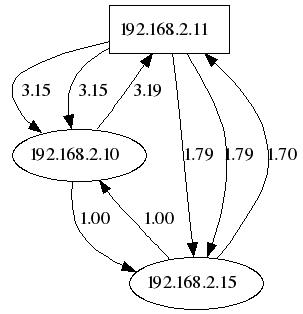
\includegraphics[width=0.5\textwidth]{images/Topology.jpg}
\caption{Topologie dargestellt mit dem olsr.org Plugin \textbf{dot\_draw}}
\label{fig:Topology}
\end{figure}

\todo{Bedeutung der Zahlen?}

\subsubsection{Routing-Tabelle}

Auf dem Bild \ref{fig:httpinfo} kann man die Routing-Tabelle
eines Linux-Rechners betrachten

\begin{figure}[H]
\centering
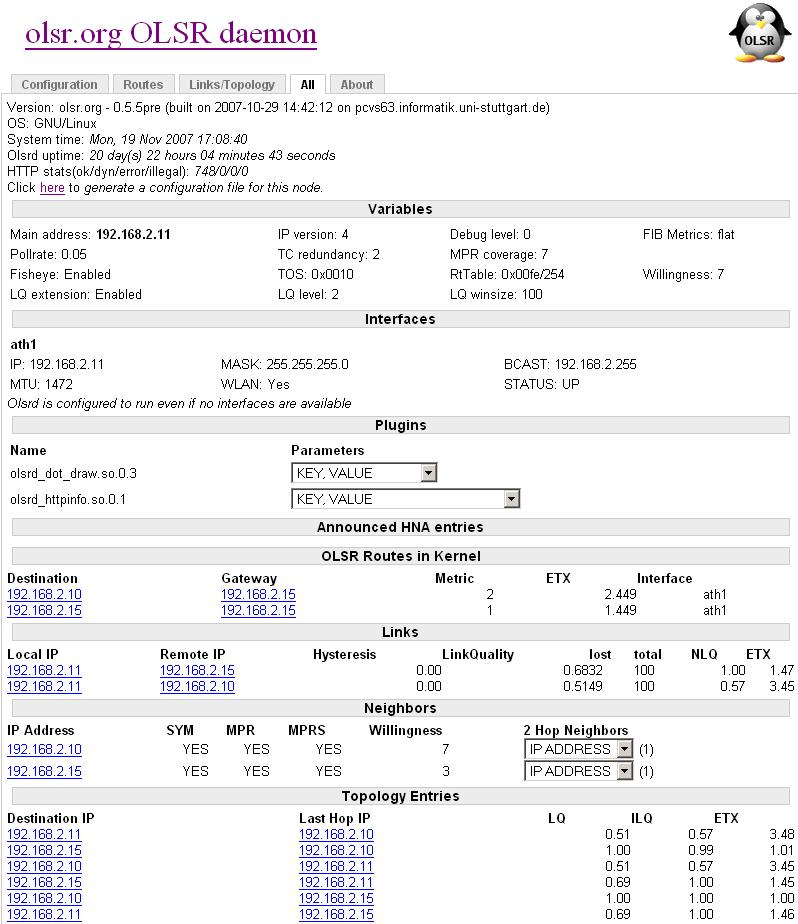
\includegraphics[width=1.0\textwidth]{images/Olsr_Route.jpg}
\caption{Routing-Tabelle eines Knotens dargestellt
	mit dem olsr.org Plugin \textbf{httpinfo}}
\label{fig:httpinfo}
\end{figure}
